\documentclass{article}
\usepackage[utf8]{inputenc}
\usepackage{amsmath}
\usepackage{amsfonts}
\usepackage{graphicx}


\begin{document}

\title{Solution to Problem of the day.}
\author{Prajit Adhikari}
\maketitle

4. Triangle ABC is given such that $\angle C = 90$. consider points $D$ on side $AC$ and $K$ on side $BD$ such that $\angle ABC = \angle KAD = \angle AKD$. Prove that $BK = 2DC$.\\

Solution:\\

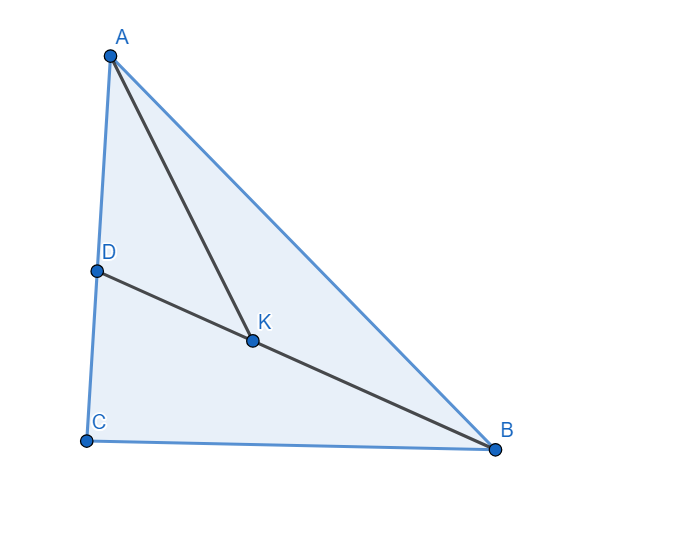
\includegraphics[width=\textwidth]{geo.PNG}
Let, $\angle ABC=x$
Angle chasing:
$$\angle CDB =2x \text{[Exterior angle]}, \angle DCB= 90^o -2x$$
$$\angle AKB = 180^o-x, \angle KAB=90^o-2x$$
Using sine law, on triangle $ABC$, we get,
$$\frac{AB}{\sin{90^o}}=\frac{BC}{\cos{x}} \implies BC=AB \cos{x} $$

Using sine law, on triangle $DBC$,
$$\frac{DC}{\cos{2x}}=\frac{BC}{\sin{2x}} \implies AB= \frac{DC.2sin{x}} {\cos{2x}}$$
Then,Using sine law, on triangle $ABK$, we get,
$$ \frac{AB}{\sin{x}}=\frac{BK}{\cos{2x}}$$
Substituting $AB$, we get,
$$\frac{2.DC.\sin{x}}{\cos{2x}.\sin{x}}=\frac{BK}{\cos{2x}}$$
$$\boxed{BK=2DC}$$
QED.






















\end{document}